\def\year{2017}\relax
%File: formatting-instruction.tex
\documentclass[letterpaper]{article} %DO NOT CHANGE THIS
\usepackage{aaai17}  %Required
\usepackage{times}  %Required
\usepackage{helvet}  %Required
\usepackage{courier}  %Required
\usepackage{url}  %Required
\usepackage{graphicx}  %Required
\usepackage[ruled,vlined]{algorithm2e}
\frenchspacing  %Required
\setlength{\pdfpagewidth}{8.5in}  %Required
\setlength{\pdfpageheight}{11in}  %Required
%PDF Info Is Required:
  \pdfinfo{
/Title (Supervised Reinforcement Learning with Partial States: a Teaching Method for Action Selection for HRI)
/Author (Emmanuel Senft)}
\setcounter{secnumdepth}{0}  
 \begin{document}
% The file aaai.sty is the style file for AAAI Press 
% proceedings, working notes, and technical reports.
%
\title{Supervised Reinforcement Learning with Partial States: \\
 a Teaching Method for Action Selection for HRI}

\author{Emmanuel Senft \and S\'{e}verin Lemaignan\\
Centre for Robotics and Neural Systems \\
Plymouth University \\
United Kingdom\\
\And Paul Baxter\\
L-CAS\\
University of Lincoln\\
United Kingdom\\
 \And Tony Belpaeme\\
 CNRS\\ Plymouth University (UK) \\ iMinds \\ Ghent University (Be)}

\maketitle
\begin{abstract}
Robots are expected to be pervasive in human society in the future

not possible to hardcode everything by hand

requirement for learning

hard to learn for HRI
\begin{itemize}
	\item real time
	\item cost of exploration (real humans)
	\item no clear reward policy and cannot request a human to reward everything
	\item need to make the most out of each sample
\end{itemize}

Partial state RL - accelerate learning


\end{abstract}
%===============================================================================

\section{Introduction}

Human-Robot Interaction (HRI) aims at having humans and robot living together
in the society, interacting socially in many different environments and
contexts. Robot are expected to behave appropriately regardless of the domain
of interaction. However, not all behaviours are known in advance and can be
implemented in the robot before its deployment in the real world. Robots need
to be able to learn new tasks, new actions policies, new social norms and how
to make sense of the world surrounding them.

When interacting in the real world, humans face huge spaces of almost unlimited
dimensions, and despite this complexity, adults and even more children are able
to learn quickly, often from only a few demonstrations or examples. Humans are
able to take the most out of every datapoint availble to them. On the other
hand, recent advances in Machine Learning such as Deep Learning \cite{lecun2015deep}
have been made possible by the availability of huge dataset covering millions
of labeled examples or dozens of hours recording. These progress have
targetting either perception, where labeled datapoints can be available or
action selection in virtual environments where the impact of actions is
limited.

Similarly to humans, robots interacting in the real world will have to be able
to learn quickly, from different types of inputs: demonstrations, commands,
rewards and also autonomously.


State used for action selection can be from different sensors, continuous, discrete, representing a value or a state

\cite{kober2013reinforcement}
%===============================================================================

\section{Background}
\subsection{Reinforcement Learning}

The main framework to provide a robot with autonomous learning is Reinforcement
Learning (RL)(\cite{kober2013reinforcement,sutton1998reinforcement}. The main idea
behind reinforcement learning is that a agent is interacting in an environment
providing positive or numerical reward in reaction to the agent's actions and
the agent selects actions to maximise the expected cummulative discounted
reward. 

Classic approaches RL relies on exploring virtual environments where the agent
tries to maximise the reward, but where in the end exploration often do not
have a real impact and where the agent can interact as long as needed to gather
enough information on the environment to find a correct action policy.

But in many real worl problem, relying only on random exploration to obtain
knowledge on the environment is not enough, the agent needs to have some initial
knowledge or additional knowledge provided often by humans to  work more
efficiently and achieve more complex results.

\subsection{Human enhanced Reinforcement Learning}
\subsubsection{Initial knowledge}
One way to use human knowledge to help an agent to learn is through providing
initial knowledge. 
alphago

IRL

OpenAI deep RL

One of the main challenge when applying RL to robotics is poor perfermance in
the early stages of the learning as the agent has to explore the environment to
gather initial knowledge. This challenge is especially
important for robotics as trials often have to happen in the real world (as
simulator close enough to the real world as not available) and as such can
present risks for the robot or for the persons interacting with it. 

\subsubsection{Guiding the learning}
scafolding 
shaping
guidance

%===============================================================================

\section{Proposition}
\subsection{Supervised Progressively Autonomous Robot Competencies}

As a way to enable a human supervisor to teach a robot an action policy while
interacting with its environment, we proposed the Supervised Progressively
Autonomous Robot Competencies (SPARC) in \cite{senft2015sparc}. SPARC is independent
of the learning algorithm used, but define an interaction dynamic between an
agent learning an action policy while interacting in an environment and a
supervisor teaching this agent an action policy. The main goal of SPARC is
enabling a robot to learn from a supervisor while ensuring that every action
executed by the robot has approval of the supervisor but without requiring this
supervisor to manually enforce every single action.

The main concept in SPARC is giving the supervisor the control over the agent
action and combine this with online learning on the agent side. This control is
achieved using a suggestion/correction mechanism whereas the agent is presenting
to the supervisor the action about to be executed and the supervisor can cancel
this action before its execution or not doing anything, letting the action being
executed after a delay. Additionally, the supervisor can select actions to be
executed by the agent. The actions selected or canceled by the supervisor can be
used as input with the current state by a learning algorithm to progressively
improve the future suggestions.

Giving power to an expert to correct the actions of the agent before the
execution can ensure that even in the early phases of the learning the agent can
have an appropriate action policy for the current environment as shown in Figure~\ref{fig:comparison}.

\begin{figure}
    \centering
    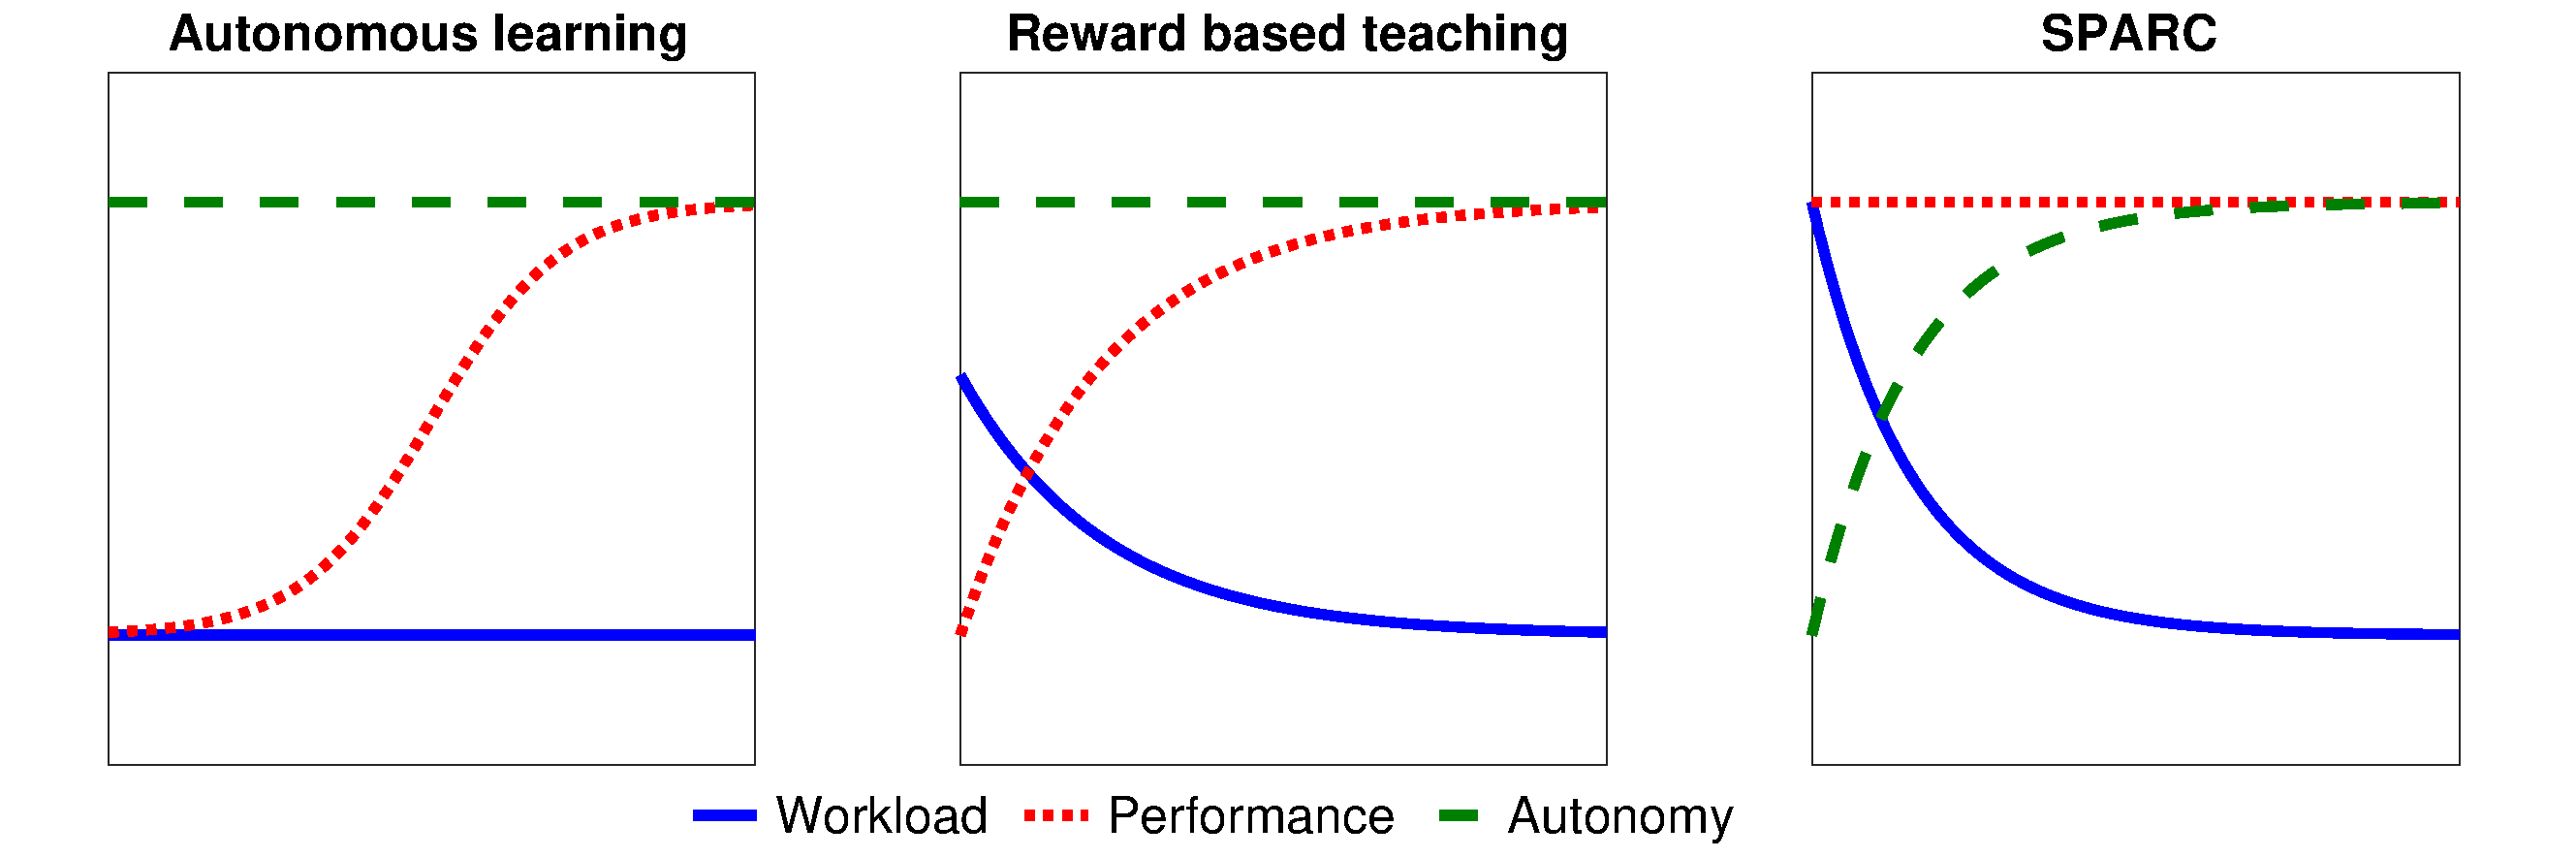
\includegraphics[width=0.9\linewidth]{./fig/motivation.pdf}
    \caption{Idealised expectation for performance, autonomy and workload for a
    Wizard of Oz, a autonomous learner and SPARC.}
    \label{fig:comparison}
\end{figure}

SPARC has been design with the idea of teaching a robot to interact with humans,
it is specially usefull when the pace of action selection is low (less than
1Hz), when the agent has to learn with a limited number of datapoints and when
undesired actions executed by an agent can have a high cost. 

In \cite{senft2017supervised}, we presented a way to combine SPARC and RL, by
assigning a positive reward to every action executed by the robot as it would
have been passively or actvely validated by the supervisor. However this method
was not making use of any type of generalisation, it was directly mapping a
single state action pair to a reward. 

\subsection{Partial-State Supervised Reinforcement Learning}

REFORMULATE: start with size of the world
To be usable in complex environments, a
learning algorithm requires generalisation as exactly identical spaces might
never been observed twice.

A classical approach to generalise in RL is to use a first layer of neural
network or to use deep reinforcement learning which relies on deep neural
networks to learn a mapping state-action-Qvalue for example. (ADDREF)
These approaches, neural network based, relies on having a large number of
datapoints to converge toward a good function approximator. However, as
discussed previously, in many application, these amounts of data are not
possible to be obtained and a robot might need to adapt to different persons and
be retrained quickly.

With that idea in mind, we propose to make a better use of human inputs, and ask
 the supervisor to identify which features of the environment are linked to the
 current selected action. That was, instead of having an state-action pair, we
 can have a partial-state action pair, with this partial-state being a subset of
 the state domain.

%===============================================================================
\section{Methodology}

\subsection{Supervisation}
Similarly to a SPARC setup, the supervisor is presented with action about to be
executed by the robot and can either cancel it or let it be executed and the 
supervisor has the possibility to select actions for the robot to execute.

In addition to these actions, the supervisor can use the GUI to select features
of the environment that can send to the algorithm to reduce the state associated
to this action to a partial-state. Similarly, the algorithm can indicate which
parts of the states have been used for the selection to the supervisor who can
correct them while the action is being executed.

Example?

\subsection{Learning algorithm}

In a first approach, the presence of an expert supervisor who can evaluate the
expected future impacts of an action removes the problem of credit assignment
for delayed rewards and allows us to consider only a myopic approach. (can cite
kobers I think.)

For this paper, we will reuse the formalism of rewardless Markov Decision 
Process to identify the different elements of our system. The agent has action
to a set of actions A, a state S (represented as a vector of n dimensions of
values $\in [0;1]$). With each dimension of S representing features in the
environment.

At the state $s_{t}$ the agent receives the action $a_{i}$ with the partial
state $s'$ defined in a subspace $S' \subseteq S$ (defined by selecting only a
number $n' \leq n$ of the dimensions of S). For example, a state s could be
defined in 4 dimensions such as $s=[1,0.2,0,0.5]$, and s' in two dimensions with
$s'=[-,0.2,0,-]$ with symbol '-' reprensenting the dimensions removed.

We store in memory the partial-state action pair $s'-a_{i}$, with the reward 1
as the action has been selected by the supervisor. Similarly, if an action has
been canceled by the supervisor, the partial-state action will be assigned to a
reward $-1$.

After interacting with the system under the supervisors control, the actions
will have associated to each action $a \in A$, a collection $C_{a}$ of pairs
partial-state-reward. When facing a new state $s$ where an action has to be
selected, the agent can select an action following Algorithm \ref{algo}.

\begin{algorithm}
    \DontPrintSemicolon
    \SetKwInOut{Input}{inputs}\SetKwInOut{Output}{output}
    \Input{Current state s, action-partial state rewards tuples}
    \Output{selected action $\pi(s)$}
    \ForEach{a $\in$ A}{
        \ForEach{s'-r $\in C_{a}$}{
            compute similarity
            $\Delta(s',s)=1-\frac{\sum_{j}^{n'}(s'(j)-s(j))^{2}}{n'}$
        }
        $\Delta(a)=max(\Delta)$

        $r(a)=R(argmax_{s'} \Delta(s'))$
    }
    $\pi(s) = argmax_{a}\Delta(a) \cdot r(a)$

    \caption{Algorithm for selecting an action based on previous
    partial-state action rewards tuples and current state}
    \label{algo}
\end{algorithm}

When proposing an action following Algorithm~\ref{algo}, the agent can also use
the dimensions of the similar state s' to indicate the supervisor which parts of
the states have been used for the action selection.

%===============================================================================
\section{Challenges}

The main challenge for using Interactive Machine Learning is to translate the
state-action space between the human view and the algorithm view. This is one
important reason why many researchers in IML focuse on limiting the human impact
to providing reward~\cite{knox2009interactively} or kinesthetic demonstrations
in the robot space~\cite{billard2008robot}. However as shown by Thomaz and Breazeal~\cite{thomaz2008teachable}, using more complex inputs from the supervisor, such
as guidance biasing the action selection can lead to a better performance in the
learning. But to able to use these higher level and more complex inputs from
humans, these actions have to be translated in inputs usable for the learning
algorithm and/or the action selection mechanism. 

The more complex the inputs from the humans are the more additional information
can be transmitted to the learning, allowing the agent to learn more complex
behaviours faster.

Similarly, as shown by Senft and al. in \cite{senft2017supervised}, providing
more control to the supervisor about the robot actions can lead to keep the
agent in relevant states of the environment and as such speeding the learning
and making it safer for the robot and people interacting with it. However this
method is dependent of letting the human know what action the robot is about to
execute, which relies on the robot to express its intention in a human
understandable way. (ADDREF - see Serge?)

Another challenge is state representation, the state accessed by the learning
algorithm and the one accessed by the supervisor can be represented is highly
different space, covering different features, and if the robot aims to profit
from the human initial knowledge, it needs to have access to similar features in
the environment to the ones the human is using, and the human needs to be able
to transmit these features to the learning algorithm.
(the representation of the state is often engineered by the programmers of the
algorithm, and space features not considered in the initial design could
actually be important in the final one. Idea of Deep Learning, but not enough
datapoints.)

Needs a parallel to human learning from humans

\section{Future work}

This method still has to be tested in a real Human-Robot Interaction, and this
evaluation is currently being implemented and will be tested in a near future.

Other way of extending the current work would be to combine it with the
possibility of letting the agent continue to explore in the absence of a
supervisor around a learnt action policy to keep improving its behaviour. This
could be done by allowing the supervisor to provide rewards during the learning
phase, rewards which could also be assigned to partial states. The system could
also learn to predict these rewards in an approach similar to TAMER 
\cite{knox2009interactively}. But in the case of an absence of supervisor, the assumption that only a
myopic action selection is sufficient would not hold anymore and the problem of
delayed rewards would have to be tackled. It could be for example possible to
adapt well known algorithms such as QLearning to handle partial states rather
the full states.

%===============================================================================
\section{Conclusion}
\label{sec:conclusion}
%==============================================================================
\section{Acknowledgments}
This work was supported by the EU FP7 DREAM project (grant no.  611391) and EU
H2020 Marie Sklodowska-Curie Actions project DoRoThy (grant 657227).  

\bibliographystyle{aaai} \bibliography{biblio}
\end{document}
